\section{Ruang $CAT_p(0)$}
Sebelum membahas mengenai ruang $CAT_p(0)$, terlebih dahulu dikenalkan ruang $CAT(0)$, sebab ruang $CAT_p(0)$ adalah perumuman dari ruang $CAT(0)$. Ruang $CAT(0)$ sejatinya adalah ruang geodesik, tetapi dengan syarat tambahan bahwa setiap segitiga geodesik di ruang tersebut memenuhi ketaksamaan $CAT(0)$. Untuk itu, berikut diberikan konsep dari segitiga komparasi. 

% segitiga geodesik lebih ramping daripada segitiga pembanding di $\mathbb{R}^2$. Untuk itu berikut diberikan konsep dari segitiga komparasi. 
\begin{defn}\cite{Bridson1999}
    Diberikan segitiga geodesik $\triangle (p,q,r)$ pada ruang metrik geodesik $(X,d)$. Suatu segitiga komparasi $\overline{\triangle}(\overline{p},\overline{q},\overline{r})$ adalah suatu segitiga di ruang bernorma $(\mathbb{E},\|\cdot\|)$ yang memenuhi $d(p,q)=\|\overline{p}-\overline{q}\|, d(p,r)=\|\overline{p}-\overline{r}\|$, dan $d(q,r)=\|\overline{q}-\overline{r}\|$.
\end{defn}
\begin{exam}\label{con:segkom}\cite{Eskandani2018}
    Diberikan ruang metrik $(\mathbb{R}^2,\tilde{d})$ dengan metrik $\tilde{d}$ yang didefinisikan untuk setiap $x=(x_1,x_2), y=(y_1,y_2)\in \mathbb{R}^2$ sebagai 
    \begin{align*}
        \tilde{d}(x,y) = \sqrt{(x_1 - y_1)^2 + \qty(x_1^2-x_2 + y_2-y_1^2)^2}.
    \end{align*}
    Ruang metrik tersebut adalah ruang metrik geodesik dengan geodesik yang menghubungkan $x$ dan $y$ didefinisikan sebagai
    \begin{align*}
        G(t) = \left((1-t)x_1 + ty_1, \qty((1-t)x_1 + ty_1)^2-(1-t)(x_1^2-x_2)-t(y_1^2-y_2)\right),
    \end{align*}
    untuk setiap $t\in [0,1]$.
    Untuk setiap segitiga geodesik $\triangle(p,q,r)$ dengan $p=(p_1,p_2)$, $q=(q_1,q_2)$, dan $r=(r_1,r_2)\in(\mathbb{R}^2,\tilde{d})$, segitiga komparasi $\overline{\triangle}(\overline{p},\overline{q},\overline{r})$ di ruang Euclid $(\mathbb{R}^2,\|\cdot\|_2)$ dapat dibentuk dengan memilih titik $\overline{p}=(p_1,p_1^2-p_2)$, $\overline{q}=(q_1,q_1^2-q_2)$, $\overline{r}=(r_1,r_1^2-r_2)\in \mathbb{R}^2$ sehingga berlaku  
    \begin{align*}
        \tilde{d}(p,q) &= \sqrt{(p_1 - q_1)^2 + \qty(p_1^2-p_2 + q_2-q_1^2)^2} = \|\overline{p}-\overline{q}\|_2,\\
        \tilde{d}(p,r) &= \sqrt{(p_1 - r_1)^2 + \qty(p_1^2-p_2 + r_2-r_1^2)^2} = \|\overline{p}-\overline{r}\|_2,\\
        \tilde{d}(q,r) &= \sqrt{(q_1 - r_1)^2 + \qty(q_1^2-q_2 + r_2-r_1^2)^2} = \|\overline{q}-\overline{r}\|_2.
    \end{align*}
\end{exam}
Selanjutnya, berikut ini diberikan definisi ruang $CAT(0)$.
\begin{defn}\cite{Bridson1999}
    Diberikan ruang metrik geodesik $(X,d)$ dan ruang Euclid $(\mathbb{R}^2,\|\cdot\|_2)$. Ruang $(X,d)$ disebut sebagai ruang $CAT(0)$ jika untuk setiap segitiga geodesik $\triangle(p,q,r)\in X$ dan $x,y\in \triangle(p,q,r)$, terdapat segitiga komparasi $\overline{\triangle}(\overline{p},\overline{q},\overline{r})\in \mathbb{R}^2$ sehingga untuk setiap $\overline{x},\overline{y}\in\overline{\triangle}$ berlaku $d(x,y)\leq \|\overline{x}-\overline{y}\|_2$.
\end{defn}
\begin{exam}
    Sebagaimana Contoh \ref{con:segkom}, ruang metrik geodesik $(\mathbb{R}^2,\tilde{d})$ adalah ruang $CAT(0)$ karena untuk setiap segitiga geodesik $\triangle(p,q,r)$ di $(\mathbb{R}^2,\tilde{d})$ dan $x,y\in \triangle(p,q,r)$, terdapat segitiga komparasi $\overline{\triangle}(\overline{p},\overline{q},\overline{r})$ di ruang Euclid $(\mathbb{R}^2,\|\cdot\|_2)$ sehingga untuk setiap $\overline{x},\overline{y}\in \overline{\triangle}(\overline{p},\overline{q},\overline{r})$ berlaku $d(x,y)\leq \|\overline{x}-\overline{y}\|_2$.
\end{exam}
\begin{exam}\cite{Bridson1999}\label{con:hilbert}
    Setiap ruang Hilbert adalah ruang $CAT(0)$.
\end{exam}

% \begin{figure}
%     \centering
%     \begin{tikzpicture}[scale=1.1, line cap=round, line join=round]

% =====================
% Gambar kiri
% =====================
\begin{scope}
% Titik-titik
\path (0,0) coordinate (p) (2.4,2.2) coordinate (q) (4.2,0.3) coordinate (r);
\path (1.0964,0.726) coordinate (A) (2.075,0.427) coordinate (B);

% Segitiga utama
\draw (p) arc(-90-15+42.51:-90+15+42.51:{3.256/(2*sin(15))}) -- (q);
\draw (r) arc(90-15+4.0856:90+15+4.0856:{4.21/(2*sin(15))}) -- (p);
\draw (q) arc(-90-15-46.5481577:-90+15-46.5481577:{2.617/(2*sin(15))}) -- (r);


% Garis dalam
% \draw (A) arc(-90-15-16.99:-90+15-16.99:{1.02325/(2*sin(15))});
\draw (A) -- (B);

% Titik
\fill (p) circle (1.5pt) node[below left] {$p$};
\fill (q) circle (1.5pt) node[above] {$q$};
\fill (r) circle (1.5pt) node[below right] {$r$};

\fill (A) circle (1.5pt) node[above left] {$x$};
\fill (B) circle (1.5pt) node[below right] {$y$};

% Tanda ruas sama panjang
\end{scope}

% =====================
% Gambar kanan
% =====================
\begin{scope}[xshift=6cm]
% Titik-titik
\coordinate (pb) at (0,0);
\coordinate (qb) at (2.4,2.2);
\coordinate (rb) at (4.2,0.3);

\coordinate (xb) at (0.4*2.4,0.4*2.2);
\coordinate (yb) at (0.5*4.2,0.5*0.3);

% Segitiga utama
\draw (pb)  --(qb) --(rb)--cycle;

% Garis dalam
\draw (xb)--(yb);

% Titik
\fill (pb) circle (1.5pt) node[below left] {$\overline{p}$};
\fill (qb) circle (1.5pt) node[above] {$\overline{q}$};
\fill (rb) circle (1.5pt) node[below right] {$\overline{r}$};

\fill (xb) circle (1.5pt) node[above left] {$\overline{x}$};
\fill (yb) circle (1.5pt) node[below right] {$\overline{y}$};

% Tanda ruas sama panjang
\end{scope}

\end{tikzpicture}

%     \caption{Caption}
%     \label{fig:placeholder}
% \end{figure}
% \begin{tikzpicture}[
%     year/.style={
%         rectangle,
%         rounded corners,
%         draw=black,
%         fill=#1,
%         minimum width=2.8cm,
%         minimum height=0.9cm,
%         font=\bfseries,
%         align=center
%     },
%     desc/.style={
%         align=left,
%         font=\small,
%         text width=10cm
%     },
%     arrow/.style={
%         thick, ->, >=stealth
%     }
% ]

% % Nodes Tahun
% \node[year=cyan!40] (y2025) at (0,0) {$\dots$ - 2025};
% \node[year=red] (mulai) at (0, -2) {mulai};
% \node[year=blue!55] (y2026) at (0,-3.8) {2026};
% \node[year=red] (selesai) at (0,-5.6) {selesai};
% \node[year=cyan!40] (y2027) at (0,-7.6) {2027};
% \node[year=cyan!40] (y2028) at (0,-9.6) {2028};
% \node[year=cyan!40] (y2029) at (0,-11.6) {2029};
% \node[year=cyan!40] (y2030) at (0,-13.6) {2030};

% % Deskripsi
% \node[desc] at (7,0) {
% Aproksimasi titik tetap dari pemetaan nonekspansif di ruang Banach.
% };

% \node[desc] at (7,-2) {
% Studi pendahuluan (proposal)
% };
% \node[desc] at (7,-3.8) {
% - Konvergensi skema iterasi Sabri untuk pemetaan $(\alpha,\beta,\gamma)$-nonekspansif di ruang CAT$_p(0)$.\\
% - Aplikasi pada rekonstruksi gambar.

% };
% \node[desc] at (7,-5.6) {
% Submit hasil penelitian ke jurnal Scopus peringkat Q2, naskah tesis, dan penyusunan laporan akhir. 
% };

% \node[desc] at (7,-7.6) {
% Pengembangan skema iterasi Sabri dan perbandingan laju konvergensi secara analitik.
% };

% \node[desc] at (7,-9.6) {
% Aplikasi skema iterasi Sabri pada pelacakan kendali gerak robot berlengan ganda.
% };

% \node[desc] at (7,-11.6) {
% Aplikasi skema iterasi Sabri pada permasalahan pemulihan sinyal.
% };

% \node[desc] at (7,-13.6) {
% Generalisasi aproksimasi titik tetap pada ruang geodesik nonlinier lainnya.
% };

% % Panah
% \draw[arrow] (y2025) -- (mulai);
% \draw[arrow] (mulai) -- (y2026);
% \draw[arrow] (y2026) -- (selesai);
% \draw[arrow] (selesai) -- (y2027);
% \draw[arrow] (y2027) -- (y2028);
% \draw[arrow] (y2028) -- (y2029);
% \draw[arrow] (y2029) -- (y2030);

% \end{tikzpicture}
% \begin{tikzpicture}[
%     >=stealth,
%     main/.style={draw, fill=blue!15, rounded corners, align=center, font=\small},
%     box/.style={draw, fill=red!10, rounded corners, align=center, font=\small},
%     line/.style={thick}
% ]

% % Spine
% \draw[line] (0,0) -- (12,0);

% % Head
% \node[main, minimum width=2cm, minimum height=1cm] 
%     at (12,0) {Aproksimasi titik tetap\\ dari pemetaan \\$(\alpha,\beta,\gamma)$-nonekspansif\\ di ruang $CAT_p(0)$ \\beserta aplikasinya};

% % === Upper bones ===
% % Pemetaan nonekspansif
% \draw[line] (3,0) -- (2,4);
% \node[box, minimum height=1cm, minimum width=2.5cm] at (1.3,4.5)
% {Pemetaan nonekspansif\\ diperumum
% % mencakup lebih banyak pemetaan 
% % aplikasi lebih luas
% % hasil terbaru abcnonekspansif
% % Suzuki\\
% % Reich--Suzuki\\
% % $(\alpha,\beta,\gamma)$-nonekspansif\\
% % Skema iterasi Sabri
% };
% \node at (0,1) {Suzuki};

% % Ruang geodesik
% \draw[line] (8,0) -- (6.5,2);
% \node[box, minimum width=4cm] at (6,2.4)
% {Ruang Geodesik
% % \footnotesize
% % struktur nonlinear 
% % hasil terbaru ruang cat_p
% % Ruang CAT(0)\\
% % Ruang CAT$_p$(0)\\
% % Struktur nonlinier\\
% % Konveksitas geodesik
% };

% % === Lower bones ===
% % Urgensitas
% \draw[line] (4,0) -- (1.3,-4.3);
% \node[box, minimum width=4.5cm] at (6,-4.6)
% {Urgensitas Penelitian
% % \footnotesize
% % Keterbatasan hasil di ruang Banach\\
% % Minimnya studi di CAT$_p$(0)\\
% % Kebutuhan skema iterasi yang efisien
% };

% % Aplikasi
% \draw[line] (8,0) -- (6,-4.2);
% \node[box, minimum width=4cm] at (1,-4.6)
% {Aplikasi Optimasi
% % \footnotesize
% % Rekonstruksi gambar\\
% % Masalah minimisasi konveks\\
% % Formulasi sebagai titik tetap\\
% };

% \end{tikzpicture}


Khamsi mengembangkan ruang yang lebih umum, yaitu ruang $CAT_p(0)$, dengan $p\geq 2$, dengan mengganti segitiga komparasi pada ruang $CAT(0)$ dari yang awalnya segitiga di $\mathbb{R}^2$ menjadi segitiga di $\ell_p$. Berikut ini definisi dari ruang $CAT_p(0)$. 
\begin{defn}\cite{Khamsi2017}\label{defn:catp0}
    Diberikan ruang metrik geodesik $(X,d)$ dan ruang $(\ell_p,\|\cdot\|_p)$ untuk $p\geq 2$. Ruang $(X,d)$ disebut sebagai ruang $CAT_p(0)$, untuk $p\geq 2$, jika untuk setiap segitiga geodesik $\triangle(p,q,r) \in X$ dan $x,y\in\triangle(p,q,r)$, terdapat segitiga komparasi $\overline{\triangle}(\overline{p},\overline{q},\overline{r})\in \ell_p$ sehingga untuk setiap $\overline{x},\overline{y}\in \overline{\triangle}$ berlaku $d(x,y)\leq \|\overline{x}-\overline{y}\|_p$.
\end{defn}
\begin{exam}\cite{Khamsi2017}
    Ruang $CAT(0)$ adalah ruang $CAT_p(0)$ dengan $p=2$.
\end{exam}
\begin{exam}\cite{Khamsi2017}\label{con:lpcatp}
Setiap ruang $(\ell_p, \|\cdot\|_p)$ dengan $p\geq 2$ adalah ruang $CAT_p(0)$. 
\end{exam}
Penjelasan dari Contoh \ref{con:lpcatp} adalah sebagai berikut.

Diketahui bahwa setiap ruang $(\ell_p, \|\cdot\|_p)$ dengan $p\geq 2$ adalah ruang metrik geodesik. Misalkan $\triangle(p,q,r)$ adalah segitiga geodesik di $(\ell_p, \|\cdot\|_p)$ dengan $p,q,r\in \ell_p$ dan $x,y\in \triangle(p,q,r)$. Dapat dipilih segitiga komparasi $\overline{\triangle}(\overline{p},\overline{q},\overline{r})\in (\ell_p, \|\cdot\|_p)$ dengan $\overline{p}=p$, $\overline{q}=q$, dan $\overline{r}=r$ sehingga untuk setiap $\overline{x},\overline{y}\in \overline{\triangle}$ berlaku $\overline{x}=x$ dan $\overline{y}=y$. Dengan demikian, diperoleh
\begin{align*}  
    d(x,y) &= \|x-y\|_p = \|\overline{x}-\overline{y}\|_p,
\end{align*}
yang menunjukkan bahwa ruang $(\ell_p, \|\cdot\|_p)$ dengan $p\geq 2$ adalah ruang $CAT_p(0)$.

Selanjutnya, berikut ini diberikan sebuah lema yang menyatakan bahwa ruang $CAT_p(0)$ dengan $p>2$ bukan merupakan ruang $CAT(0)$.
\begin{lemma}\cite{Khamsi2017}\label{lema:p=2}
Untuk $p>2$ ruang $CAT_p(0)$ bukan merupakan ruang $CAT(0)$.
\end{lemma}

Berikut ini diberikan sebuah contoh ruang $CAT_p(0)$ dengan $p=3$ yang bukan merupakan ruang Banach dan bukan pula ruang $CAT(0)$.

    \begin{exam}\label{con:Catp}
    Diberikan $X=\{(x_1,x_2,\cdots)~|~x_i\in \mathbb{R}, \sum_{i=1}^{\infty} |x_i|^3<\infty\}$ dan untuk setiap $x=(x_1,x_2,x_3,\cdots),y=(y_1,y_2,y_3,\cdots)\in\ell_3$ didefinisikan metrik
    \begin{align}\label{eq:conMetrik}
    d(x,y)=\left(|x_1-y_1|^3+|x_1^3-x_2-y_1^3+y_2|^3+\sum_{i=3}^{\infty}|x_i-y_i|^3\right)^{\frac{1}{3}}.
    \end{align}
    Didefinisikan pula geodesik yang menghubungkan $w=(w_1,w_2,w_3,\dots)$ dan $z=(z_1,z_2,z_3,\dots)$, yaitu $G:[0,1]\to X$ dengan $G(t):=(1-t)w\oplus tz$ sebagai
    \begin{align}\label{eq:conGdsk}
    G(t)=\big(\alpha_1(t), \alpha_1(t)^3-(1-t)(w_1^3-w_2)-t(z_1^3-z_2),\alpha_3(t),\alpha_4(t),\cdots\big),
    \end{align}
    dengan $\alpha_i(t)=(1-t)w_i+tz_i$ untuk $i=1,3,4,5,\cdots$.\\
    Ruang $(X,d)$ merupakan ruang $CAT_p(0)$, tetapi bukan ruang Banach dan bukan ruang $CAT(0)$.
    \end{exam}
    Penjelasan dari Contoh \ref{con:Catp} dapat diuraikan sebagai berikut.\\
    Untuk setiap $x=(x_1,x_2,x_3,\dots)\in X$, didefinisikan pemetaan $M:X\to X$ sebagai $M(x)=(x_1,x_1^3-x_2,x_3,\dots)$. Pemetaan ini merupakan pemetaan bijektif yang memetakan setiap titik $x=(x_1,x_2,x_3,\dots)\in X$ ke titik lain $\overline{x}=(\overline{x_1},\overline{x_2},\overline{x_3},\dots)\in X$ dengan $\overline{x_i}=x_i$ untuk setiap $i=1,3,4,5,\dots$ dan $\overline{x_2}=x_1^3-x_2$. Diperhatikan bahwa untuk setiap $\overline{x}, \overline{y}\in X$, berlaku 
    \begin{align*}
        d(\overline{x},\overline{y}) &= \left(|x_1-y_1|^3+|x_1^3-x_2-y_1^3+y_2|^3+\sum_{i=3}^{\infty}|x_i-y_i|^3\right)^{\frac{1}{3}}\\
        &= \qty(\sum_{i=1}^{\infty} |\overline{x_i}-\overline{y_i}|^3)^{\frac{1}{3}}\\
        &= \| \overline{x}-\overline{y}\|_3.
    \end{align*}
    Hal ini menunjukkan bahwa $(X,d)$ merupakan ruang metrik yang lengkap, selanjutnya diamati bahwa 
    \begin{align*}
        G(0)=(w_1,w_2,w_3,\dots)=w \qquad \text{dan} \qquad G(1)=(z_1,z_2,z_3\dots)=z.
    \end{align*}
    Diamati pula untuk $i=1,3,4,5,\dots$
    \begin{align*}
       \beta_i (t,s)=\alpha_i(t) -\alpha_i(s)= (1-t)w_i+tz_i-\mqty((1-s)w_i+sz_i)=(s-t)(w_i-z_i)
    \end{align*}
    \allowdisplaybreaks
    serta
    \begin{align*}
        \beta_2(t,s)=~&\alpha_1(t)^3-\qty(\alpha_1(t)^3-(1-t)(w_1^3-w_2)-t(z_1^3-z_2))\\
        &-\alpha_1(s)^3+\qty(\alpha_1(s)^3-(1-s)(w_1^3-w_2)-s(z_1^3-z_2))\\
        =~& (s-t)(w_1^3-w_2-z_1^3+z_2).
    \end{align*}
    Didapatkan bahwa 
    \begin{align*}
d(G(t),G(s))&=\left(\sum_{i=1}^{\infty}|\beta_i(t,s)|^3\right)^{\frac{1}{3}} = |s-t|d(w,z).
    \end{align*}
    Hal ini berarti $G(t)$ merupakan geodesik pada $X$. Kemudian, untuk setiap segitiga geodesik $\triangle(p,q,r) \in X$ dengan $p=(p_1,p_2,p_3,\dots),q=(q_1,q_2,q_3,\dots),r=(r_1,r_2,r_3,\dots)\in X$, diperoleh bahwa terdapat segitiga komparasi $\overline{\triangle}(\overline{p},\overline{q},\overline{r})\in X$ dengan $\overline{p}=(p_1,p_1^3-p_2,p_3,\dots),\overline{q}=(q_1,q_1^3-q_2,q_3,\dots),\overline{r}=(r_1,r_1^3-r_2,r_3,\dots)$ sehingga berlaku 
    \begin{align*}
        d(p,q)&=\left(|p_1-q_1|^3+|p_1^3-p_2-q_1^3+q_2|^3+\sum_{i=3}^{\infty}|p_i-q_i|^3\right)^{\frac{1}{3}}=\|\overline{p}-\overline{q}\|_3,\\
        d(p,r)&=\left(|p_1-r_1|^3+|p_1^3-p_2-r_1^3+r_2|^3+\sum_{i=3}^{\infty}|p_i-r_i|^3\right)^{\frac{1}{3}}=\|\overline{p}-\overline{r}\|_3,\\
        d(q,r)&=\left(|q_1-r_1|^3+|q_1^3-q_2-r_1^3+r_2|^3+\sum_{i=3}^{\infty}|q_i-r_i|^3\right)^{\frac{1}{3}}=\|\overline{q}-\overline{r}\|_3.
    \end{align*}
    Selanjutnya, untuk setiap titik $x,y\in \triangle(p,q,r)$ dengan $x=(x_1,x_2,x_3,\dots),y=(y_1,y_2,y_3,\dots)$, diperoleh bahwa terdapat titik $\overline{x},\overline{y}\in\overline{\triangle}(\overline{p},\overline{q},\overline{r})$ dengan $\overline{x}=(x_1,x_1^3-x_2,x_3,\dots),\overline{y}=(y_1,y_1^3-y_2,y_3,\dots)$ sehingga berlaku 
    \begin{align*}
        d(x,y)=\left(|x_1-y_1|^3+|x_1^3-x_2-y_1^3+y_2|^3+\sum_{i=3}^{\infty}|x_i-y_i|^3\right)^{\frac{1}{3}}=\norm{\overline{x}-\overline{y}}_3.
    \end{align*}
    Jadi $(X,d)$ merupakan ruang $CAT_p(0)$ dengan $p=3$. Selanjutnya, diperhatikan bahwa 
    \begin{align*}
        d(\alpha x,0)&=\left(|\alpha x_1|^3+|(\alpha x_1)^3-\alpha x_2|^3+\sum_{i=3}^{\infty}|\alpha x_i|^3\right)^{\frac{1}{3}}\\
        &=|\alpha| \left(|x_1|^3+|\alpha^2 x_1^3-x_2|^3+\sum_{i=3}^{\infty} |x_i|^3\right)^{\frac{1}{3}}\\
        &\neq \alpha d(x,0),
    \end{align*}
    sehingga tidak bisa didapatkan norma dari metrik tersebut, yang berarti bukan ruang Banach. Berdasarkan Lema \ref{lema:p=2}, ruang ini juga bukan merupakan ruang $CAT(0)$ karena $p\neq 2$.

Diagram Venn pada Gambar \ref{fig:venncatp0} mengilustrasikan hubungan antara ruang Euclid, Hilbert, $CAT(0)$, Banach, ruang $CAT_p(0)$, dan ruang metrik geodesik.
\begin{figure}[H]
    \label{fig:venncatp0}
\centering
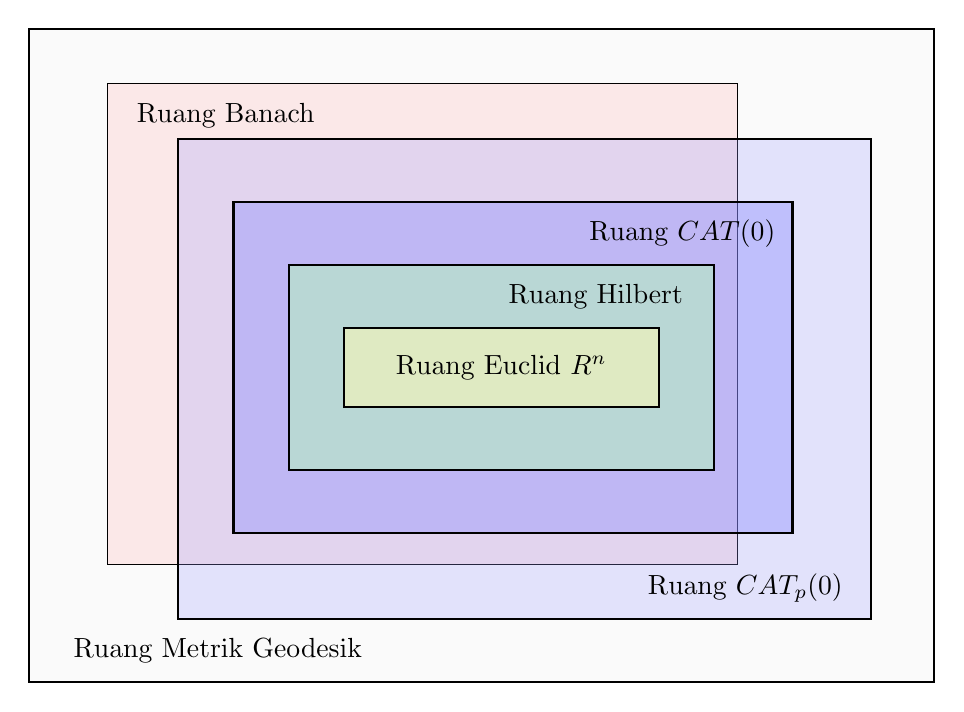
\begin{tikzpicture}

% ===== Geodesic =====
\draw[thick, fill=gray!30, fill opacity=0.12] 
    (-4,-4) rectangle (7.5,4.3);
\node at (-1.6,-3.6) {Ruang Metrik Geodesik};
%Banach
\draw[thin, fill=red!50, fill opacity=0.15] 
    (-3,-2.5) rectangle (5,3.6);
% ===== CAT_p(0) =====
\draw[thick, fill=blue!40, fill opacity=0.25] 
    (-2.1,-3.2) rectangle (6.7,2.9);

% ===== CAT(0) =====
\draw[thick, fill=blue!50, fill opacity=0.35] 
    (-1.4,-2.1) rectangle (5.7,2.1);

% ===== Banach =====



% ===== Hilbert (intersection) =====
\draw[thick, fill=green!30, fill opacity=0.45] 
    (-0.7,-1.3) rectangle (4.7,1.3);

% ===== Euclid =====
\draw[thick, fill=yellow!30, fill opacity=0.55] 
    (0,-0.5) rectangle (4,0.5);
\node at (3.2,0.9) {Ruang Hilbert};
\node at (5.1,-2.8) {Ruang $CAT_p(0)$};
\node at (4.3,1.7) {Ruang $CAT(0)$};
\node at (-1.5,3.2) {Ruang Banach};
\node at (2,0) {Ruang Euclid $\mathbb{R}^n$};

\end{tikzpicture}
\caption{\centering Hubungan antara ruang Euclid, Hilbert, $CAT(0)$, Banach, ruang $CAT_p(0)$, dan ruang metrik geodesik}
\end{figure}




 
Berikut ini diberikan beberapa konsep yang berlaku pada ruang $CAT_p(0)$ dengan $p\geq 2$.
\begin{defn}\cite{Khamsi2017} \label{defn:konveks}
    Diberikan $(X,d)$ adalah ruang $CAT_p(0)$. Suatu himpunan bagian $\mathcal{M}\subseteq X$ disebut konveks jika $[x\sim y]\subseteq \mathcal{M}$ untuk setiap $x,y\in \mathcal{M}$.
\end{defn}

Dua contoh berikut ini mengilustrasikan konsep himpunan konveks dan bukan konveks pada ruang $CAT_p(0)$.
\begin{exam}
    Dipilih ruang $CAT_p(0)$, yaitu $(\mathbb{R}^2,\tilde{d})$ pada Contoh \ref{con:segkom} dan himpunan bagian $\mathcal{M}=\{(0,b)\in \mathbb{R}^2\mid b\in \mathbb{R}\}\subset \mathbb{R}^2$. Diperhatikan bahwa untuk setiap $x=(0,x_2), y=(0,y_2)\in \mathcal{M}$, geodesik yang menghubungkan $x$ dan $y$ adalah $[x\sim y] = \{G(t)\mid t\in[0,1], G(0)=x, G(1)=y\}$ dengan
    \begin{align*}
         G(t) &= \left((1-t)0 + t0, \qty((1-t)0 + t0)^2-(1-t)(0^2 - x_2)-t(0^2 - y_2)\right)\\
         &=\left(0, (1-t)x_2 + ty_2\right).
    \end{align*}
    Karena $x_2,y_2\in \mathbb{R}$, maka $(1-t)x_2 + ty_2\in \mathbb{R}$, sehingga $[x\sim y]=\{(0, (1-t)x_2 + ty_2)\mid t\in[0,1]\}\subseteq \mathcal{M}$. Dengan demikian, himpunan bagian $\mathcal{M}$ adalah himpunan konveks di ruang $(\mathbb{R}^2,\tilde{d})$.
\end{exam}
\begin{exam}
    Dipilih ruang $CAT_p(0)$, yaitu $(\mathbb{R}^2,\tilde{d})$ pada Contoh \ref{con:segkom} dan himpunan bagian $\mathcal{M}=\{(b,0)\in \mathbb{R}^2\mid b\in \mathbb{R}\}\subset \mathbb{R}^2$. Himpunan bagian tersebut tidak konveks karena terdapat $x=(1,0), y=(-1,0)\in \mathcal{M}$ sehingga 
    \begin{align*}
        G(t) &= \left((1-t)1 + t(-1), \qty((1-t)1 + t(-1))^2-(1-t)(1^2 - 0)-t((-1)^2 - 0)\right)\\
        &=\left(1-2t, (1-2t)^2 - 1\right).
    \end{align*}
    Untuk $t=\dfrac{1}{2}$, diperoleh $G\left(\dfrac{1}{2}\right) = \left(0, -\dfrac{1}{2}\right)\notin \mathcal{M}$, sehingga himpunan bagian $\mathcal{M}$ tidak konveks di ruang $(\mathbb{R}^2,\tilde{d})$.
\end{exam}
% \todo{himpunan kompak}
% Definisi berikut ini menyatakan konsep himpunan kompak di ruang $CAT_p(0)$ yang secara langsung diadaptasi dari konsep himpunan kompak di ruang metrik pada umumnya.
% \begin{defn}
%     Diberikan $(X,d)$ adalah ruang $CAT_p(0)$. Suatu himpunan bagian $\mathcal{M}\subseteq X$ disebut kompak jika setiap barisan di $\mathcal{M}$ memiliki subbarisan yang konvergen ke suatu titik di $\mathcal{M}$.
% \end{defn}
% \begin{exam}
%     Diberikan ruang $CAT_p(0)$, yaitu $(\mathbb{R}^2,\tilde{d})$ pada Contoh \ref{con:segkom} dan himpunan bagian $\mathcal{M}=\{(x_1,x_2)\in \mathbb{R}^2\mid x_1^2 + (x_1^2-x_2)^2 \leq 1\}\subset \mathbb{R}^2$. Himpunan bagian tersebut adalah himpunan kompak karena setiap barisan di $\mathcal{M}$ memiliki subbarisan yang konvergen ke suatu titik di $\mathcal{M}$.
% \end{exam}
% Penjelasan dari contoh tersebut adalah sebagai berikut. 
% Dimisalkan $\{x_n\}\subseteq \mathcal{M}$ adalah barisan di $\mathcal{M}$ dengan $x_n=(x_{n1},x_{n2})$ untuk setiap $n\in \mathbb{N}$. 

Definisi berikut ini menyatakan konsep barisan terbatas di ruang $CAT_p(0)$ yang secara langsung diadaptasi dari konsep barisan terbatas di ruang metrik pada umumnya.
\begin{defn}
    Diberikan $(X,d)$ adalah ruang $CAT_p(0)$. Suatu barisan $\{x_n\}$ di $X$ disebut terbatas jika terdapat $B>0$ dan $M\in X$ sehingga $d(x_n,M)<B$ untuk setiap $n\in \mathbb{N}$.
\end{defn}

Pada ruang ini, konvergensi lemah yang umum digunakan pada ruang Banach digantikan dengan konsep konvergensi-$\Delta$ (Delta-convergence). Berikut ini diberikan definisi pusat asimtotik dan konvergensi-$\Delta$ di ruang $CAT_p(0)$.
\begin{defn}\cite{Salisu2022}\label{defn:asimtotik}
    Diberikan $(X,d)$ adalah ruang $CAT_p(0)$ dan $\{x_n\}$ adalah barisan terbatas di $X$. Pusat asimtotik dari barisan $\{x_n\}$ di suatu $CAT_p(0)$ didefinisikan sebagai 
    \begin{equation}
        A(\{x_n\}) := \{x\in X\mid\limsup_{n\to\infty} d(x,x_n) = \inf_{y\in X} \limsup_{n\to \infty} d(y,x_n)\}
    \end{equation}
\end{defn}
\begin{exam}\label{con:pusasimtot}
    Diberikan ruang $CAT_p(0)$, yaitu $(\mathbb{R}^2,\tilde{d})$ pada Contoh \ref{con:segkom} dan barisan $\{x_n\}\subseteq \mathbb{R}^2$ dengan $x_n=\qty(0,(-1)^n)\in\mathbb{R}^2$ untuk setiap $n\in \mathbb{N}$. Barisan tersebut adalah barisan terbatas karena untuk setiap $n,m\in \mathbb{N}$, diperoleh
    \begin{align*}
        \tilde{d}(x_n,x_m) &= \sqrt{(0-0)^2 + \qty(0^2 - (-1)^n + (-1)^m - 0^2)^2} = |(-1)^n - (-1)^m| \leq 2.
    \end{align*}
    Selanjutnya, ditentukan pusat asimtotik dari barisan $\{x_n\}$. Diketahui bahwa untuk setiap $x=(x_1,x_2)\in \mathbb{R}^2$, berlaku
    \begin{align*}
        \limsup_{n\to\infty} \tilde{d}(x,x_n) &= \limsup_{n\to\infty} \sqrt{(x_1 - 0)^2 + \qty(x_1^2 - x_2 + (-1)^n - 0^2)^2}\\
        &= \max\left\{\sqrt{x_1^2 + (x_1^2 - x_2 + 1)^2}, \sqrt{x_1^2 + (x_1^2 - x_2 - 1)^2}\right\},
    \end{align*}
    sehingga diperoleh
    \begin{align*}
        \inf_{y\in X} \limsup_{n\to\infty} \tilde{d}(y,x_n) &= \inf_{(y_1,y_2)\in \mathbb{R}^2} \max\left\{\sqrt{y_1^2 + (y_1^2 - y_2 + 1)^2}, \sqrt{y_1^2 + (y_1^2 - y_2 - 1)^2}\right\}.
    \end{align*}
    Nilai minimum dari fungsi $f(y_1,y_2)=\max\left\{\sqrt{y_1^2 + (y_1^2 - y_2 + 1)^2}, \sqrt{y_1^2 + (y_1^2 - y_2 - 1)^2}\right\}$ adalah $1$ yang terjadi pada titik $(0,0)$, sehingga
    \begin{align*}
        A(\{x_n\}) &= \{(x_1,x_2)\in \mathbb{R}^2 \mid\limsup_{n\to\infty} \tilde{d}((x_1,x_2),x_n) = 1\}= \{(0,0)\}.
    \end{align*}
    Dengan demikian, pusat asimtotik dari barisan $\{x_n\}$ adalah $\{(0,0)\}$.
\end{exam}
\begin{defn}\cite{Salisu2022}\label{defn:konvD}
    Diberikan $(X,d)$ adalah ruang $CAT_p(0)$ dan $\{x_n\}$ adalah barisan terbatas di $X$. Barisan $\{x_n\}$ disebut sebagai konvergen-$\Delta$ ke suatu titik $x\in X$ (dinotasikan $\Delta-\lim_{n\to\infty} x_n=x$) jika $\{x\}$ adalah pusat asimtotik dari setiap subbarisan $\{x_{n_k}\}$ dari $\{x_n\}$.
\end{defn}
\begin{exam}
    Diberikan ruang $CAT_p(0)$, yaitu $(\mathbb{R}^2,\tilde{d})$ pada Contoh \ref{con:segkom} dan barisan $\{x_n\}\subseteq \mathbb{R}^2$ dengan $x_n=\qty(0,\dfrac{1}{n})\in \mathbb{R}^2$ untuk setiap $n\in \mathbb{N}$. Barisan tersebut adalah barisan terbatas karena untuk setiap $n,m\in \mathbb{N}$, diperoleh
    \begin{align*}
        \tilde{d}(x_n,x_m) &= \sqrt{(0-0)^2 + \qty(0^2 - \dfrac{1}{n} + \dfrac{1}{m} - 0^2)^2} = \left|\dfrac{1}{n} - \dfrac{1}{m}\right| \leq 1.
    \end{align*}
    Selanjutnya, ditentukan pusat asimtotik dari setiap subbarisan $\{x_{n_k}\}$ dari $\{x_n\}$. Diketahui bahwa untuk setiap $x=(x_1,x_2)\in (\mathbb{R}^2,\tilde{d})$, berlaku
    \begin{align*}
        \limsup_{k\to\infty} \tilde{d}(x,x_{n_k}) &= \limsup_{k\to\infty} \sqrt{(x_1 - 0)^2 + \qty(x_1^2 - x_2 + \dfrac{1}{n_k} - 0^2)^2}\\
        &= \sqrt{x_1^2 + (x_1^2 - x_2)^2}.
    \end{align*}
    Sehingga diperoleh
    \begin{align*}
        \inf_{y\in X} \limsup_{k\to\infty} \tilde{d}(y,x_{n_k}) &= \inf_{(y_1,y_2)\in \mathbb{R}^2} \sqrt{y_1^2 + (y_1^2 - y_2)^2}.
    \end{align*}
    Nilai minimum dari fungsi $f(y_1,y_2)=\sqrt{y_1^2 + (y_1^2 - y_2)^2}$ adalah $0$ yang terjadi pada titik $(0,0)$. Dengan demikian, diperoleh
    \begin{align*}
        A(\{x_{n_k}\}) &= \{(x_1,x_2)\in \mathbb{R}^2 \mid\limsup_{k\to\infty} \tilde{d}((x_1,x_2),x_{n_k}) = 0\}\\
        &= \{(0,0)\}.
    \end{align*}
    Karena pusat asimtotik dari setiap subbarisan $\{x_{n_k}\}$ adalah $\{(0,0)\}$, maka barisan $\{x_n\}$ konvergen-$\Delta$ ke titik $(0,0)$, yaitu $\Delta-\lim_{n\to\infty} x_n = (0,0)$.
\end{exam}
\begin{exam}
    Diberikan ruang $CAT_p(0)$, yaitu $(\mathbb{R}^2,\tilde{d})$ pada Contoh \ref{con:segkom} dan barisan $\{x_n\}\subseteq \mathbb{R}^2$ dengan $x_n=\qty(0,(-1)^n)\in \mathbb{R}^2$ untuk setiap $n\in \mathbb{N}$. Sebagaimana pada Contoh \ref{con:pusasimtot}, barisan tersebut adalah barisan terbatas dan pusat asimtotik dari barisan $\{x_n\}$ adalah $\{(0,0)\}$. Kemudian, diperhatikan bahwa terdapat subbarisan $\{x_{n_k}\}$ dari $\{x_n\}$ dengan $x_{n_k}=\qty(0,1)$ untuk setiap $k\in \mathbb{N}$. Diketahui bahwa untuk setiap $x=(x_1,x_2)\in \mathbb{R}^2$, berlaku
    \begin{align*}
        \limsup_{k\to\infty} \tilde{d}(x,x_{n_k}) &= \limsup_{k\to\infty} \sqrt{(x_1 - 0)^2 + \qty(x_1^2 - x_2 + 1 - 0^2)^2}\\
        &= \sqrt{x_1^2 + (x_1^2 - x_2 + 1)^2}.
    \end{align*}
    sehingga diperoleh
    \begin{align*}
        \inf_{y\in X} \limsup_{k\to\infty} \tilde{d}(y,x_{n_k}) &= \inf_{(y_1,y_2)\in \mathbb{R}^2} \sqrt{y_1^2 + (y_1^2 - y_2 + 1)^2}.
    \end{align*}
    Nilai minimum dari fungsi $f(y_1,y_2)=\sqrt{y_1^2 + (y_1^2 - y_2 + 1)^2}$ adalah $0$ yang terjadi pada titik $(0,1)$. Dengan demikian, diperoleh
    \begin{align*}
        A(\{x_{n_k}\}) &= \{(x_1,x_2)\in \mathbb{R}^2 \mid\limsup_{k\to\infty} \tilde{d}((x_1,x_2),x_{n_k}) = 0\}\\
        &= \{(0,1)\}.
    \end{align*}
    Dengan cara yang sama dapat ditentukan pusat asimtotik dari subbarisan lain, yaitu $\{x_{m_k}\}$ dengan $x_{m_k}=\qty(0,-1)$ untuk setiap $k\in \mathbb{N}$. Pusat asimtotik dari subbarisan tersebut adalah $A(\{x_{m_k}\})=\{(0,-1)\}$. Jadi terdapat dua subbarisan dari $\{x_n\}$ yang memiliki pusat asimtotik berbeda, sehingga barisan $\{x_n\}$ tidak konvergen-$\Delta$.
\end{exam}

Untuk konvergensi kuat di ruang $CAT_p(0)$, konsepnya sama dengan konvergensi kuat di ruang metrik pada umumnya, yaitu sebagai berikut.
\begin{defn}\cite{Salisu2022}\label{defn:konvK}
    Diberikan $(X,d)$ adalah ruang $CAT_p(0)$ dan $\{x_n\}$ adalah barisan di $X$. Barisan $\{x_n\}$ disebut konvergen kuat ke suatu titik $x\in X$ (dinotasikan $\lim_{n\to\infty} d(x_n,x)=0$) jika untuk setiap $\varepsilon>0$, terdapat $n_0\in \mathbb{N}$ sehingga untuk setiap $n\geq n_0$ berlaku $d(x_n,x)<\varepsilon$.
\end{defn}
\begin{exam}
    Diberikan ruang $CAT_p(0)$, yaitu ruang $CAT(0)$ $(\mathbb{R}^2,\tilde{d})$ pada Contoh \ref{con:segkom} dan barisan $\{x_n\}\subseteq \mathbb{R}^2$ dengan $x_n=\qty(0,\dfrac{1}{n})\in\mathbb{R}^2$ untuk setiap $n\in \mathbb{N}$. Barisan tersebut konvergen kuat ke titik $x=(0,0)$ karena untuk setiap $\varepsilon>0$, dapat dipilih $n_0\in \mathbb{N}$ dengan $n_0> \frac{1}{\varepsilon}$ sehingga untuk setiap $n\geq n_0$ berlaku
    \begin{align*}
        \tilde{d}(x_n,x) &= \sqrt{(0-0)^2 + \qty(0^2 - \dfrac{1}{n} - 0^2)^2} = \dfrac{1}{n} < \varepsilon.
    \end{align*}
\end{exam}

Berikut ini diberikan definisi mengenai sifat demiclosedness pada pemetaan di ruang $CAT_p(0)$.
\begin{defn}\cite{Salisu2022}\label{defn:demi}
    Diberikan $(X,d)$ adalah suatu ruang $CAT_p(0)$. Pemetaan $T:X\to X$ disebut memiliki sifat \textbf{demiclosedness} jika untuk setiap barisan $\{x_n\}\subseteq X$ yang konvergen-$\Delta$ ke $x\in X$ dan memenuhi $\lim_{n\to \infty} d(x_n,Tx_n)=0$, maka berlaku $x=Tx$. 
\end{defn}
\begin{exam}
    Diberikan ruang $CAT_p(0)$, yaitu $(\mathbb{R}^2,\tilde{d})$ pada Contoh \ref{con:segkom} dan pemetaan $T:\mathbb{R}^2\to\mathbb{R}^2$ yang didefinisikan sebagai $T\qty((x_1,x_2)) = \left(\dfrac{x_1}{2}, \dfrac{x_2}{2}\right)$ untuk setiap $(x_1,x_2)\in \mathbb{R}^2$. Diketahui bahwa titik tetap dari $T$ adalah $(0,0)$. Misalkan $\{x_n\}\subseteq \mathbb{R}^2$ adalah barisan yang konvergen-$\Delta$ ke titik $(0,0)$ dan $\lim_{n\to \infty} d(x_n,Tx_n)=0$. Dari sini didapatkan $A({x_n})={(0,0)}$. Selanjutnya, diperhatikan bahwa 
    \begin{align*}
        \limsup _{n\to\infty} \tilde{d}\qty(T\qty((0,0)),x_{n}) &= \limsup_{n\to\infty} \sqrt{(0 - x_{n1})^2 + \qty(0^2 - 0 + x_{n2} - 0^2)^2}\\
        &= \limsup_{n\to\infty} \tilde{d}((0,0),x_n).
    \end{align*}
    Hal ini berarti, $T\qty((0,0)) \in A(\{x_n\})$ sehingga $T\qty((0,0)) = (0,0)$. Dengan demikian, pemetaan $T$ memiliki sifat demiclosedness.
   \end{exam}

   Dalam tesis ini dinotasikan $d^p(x,y)$ sebagai perkalian dari $d(x,y)$ dengan $d(x,y)$ sebanyak $p$ kali yaitu 
   \begin{align*}
    d^p(x,y) = \underbrace{d(x,y)\cdot d(x,y)\cdots d(x,y)}_{p\text{ kali}}.
   \end{align*}
   Selanjutnya, berikut ini diberikan ketaksamaan penting yang berlaku pada ruang $CAT_p(0)$. 
\begin{lemma}\cite{CALDERN2021}\label{lema:d,d^p}
    Diberikan $(X,d)$ adalah suatu ruang $CAT_p(0)$. Jika $x,y,z\in X$ dan $t\in[0,1]$, maka 
    \begin{enumerate}
        \item $d((1-t)x\oplus tz, y)\leq (1-t)d(x,y)+td(z,y)$. 
        \item $d^p((1-t)x\oplus tz, y)\leq (1-t)d^p(x,y)+td^p(z,y)-\dfrac{t(1-t)}{2^{p-1}}d^p(x,z)$.
    \end{enumerate}
\end{lemma}
% \begin{remark}\cite{CALDERN2021}
%     Suatu ruang metrik geodesik merupakan ruang $CAT_p(0)$ jika dan hanya jika memenuhi 
% \end{remark}
Lema berikut ini menyatakan keunikan pusat asimtotik dari suatu barisan terbatas di ruang $CAT_p(0)$.
\begin{lemma}\cite{Salisu2022}\label{Lema:asimtotik}
    Pusat asimtotik dari suatu barisan terbatas di ruang $CAT_p(0)$ memiliki tepat satu elemen. 
\end{lemma}
Selain itu, berikut ini diberikan teorema yang menyatakan kondisi konvergensi-$\Delta$ dari suatu barisan di ruang $CAT_p(0)$.
\begin{thm}\cite{Salisu2022}\label{thm:kondisikonvD}
    Diberikan $(X,d)$ adalah ruang $CAT_p(0)$ yang lengkap dan $W$ adalah himpunan bagian tak kosong dari $X$ yang tertutup dan konveks. Diberikan pula $T:W\to W$ adalah pemetaan yang memiliki titik tetap dan memenuhi sifat demiclosedness \ref{defn:demi}. Jika $\{x_n\}$ adalah barisan di $W$ yang memenuhi $\lim_{n\to\infty}d(x_n,Tx_n)=0$ dan barisan $\{d(x_n,x^*)\}$ konvergen di $\mathbb{R}$ untuk setiap $x^*$ titik tetap dari $T$, maka barisan $\{x_n\}$ konvergen-$\Delta$ ke titik tetap dari $T$.
\end{thm}
